    %%%%%%%%%%%%%%%%%%%%%%%%%%%%%%%%%%%%%%%%%
% Format ini disusun menyesuaikan aturan penulisan
% Structural Definitions File
%
% Ditulis Oleh: Harjito 
% Harjito@mail.unnes.ac.id
%
%
%%%%%%%%%%%%%%%%%%%%%%%%%%%%%%%%%%%%%%%%%
%----------------------------------------------------------------------------------------
%	VARIOUS REQUIRED PACKAGES
%----------------------------------------------------------------------------------------

\documentclass[a4paper,12pt]{report} 


\makeatletter
% I assume you want A4 mot US-letter, and you want chapters so report not article

%%%%%%%%%%%%%%%%%%%%%%%%%%%%%%%%%%%%%%%%
%
% Pengaturan Package
%
%%%%%%%%%%%%%%%%%%%%%%%%%%%%%%%%%%%%%%%%

\usepackage{graphicx}
\usepackage{xpatch}
\usepackage[top=4cm,bottom=3cm,left=4cm,right=3cm,headsep=10pt,a4paper]{geometry} % Page margins
\usepackage{comment}
\usepackage{titlesec}
\usepackage[titles]{tocloft} % Required for manipulating the table of contents
\usepackage{lipsum}
\usepackage{titletoc} 
\usepackage{lscape}
%\usepackage{rotating}
\usepackage{pdfpages}
\usepackage[toc,page]{appendix}

%\usepackage[nosectionbib]{apacite} 

\usepackage{xcolor} % Required for specifying colors by name
\definecolor{ocre}{RGB}{52,177,201} % Define the orange color used for highlighting throughout the book
\usepackage{indentfirst}
% Font Settings
\usepackage{times, mathptmx} % Use the Times font for headings
%\usepackage{mathptmx} % Use the Adobe Times Roman as the default text font together with math symbols from the Sym­bol, Chancery and Com­puter Modern fonts

\usepackage{microtype} % Slightly tweak font spacing for aesthetics
\usepackage[utf8]{inputenc} % Required for including letters with accents
\usepackage{csquotes}

\usepackage[T1]{fontenc} % Use 8-bit encoding that has 256 glyphs
\usepackage{titlesec}
\usepackage{scrwfile}

%%%%%%%%%%%%%%%%%%%%%%%%%%%%%%%%%%%%%%%%%%%%%%%
% Pengaturan Judul bab
%%%%%%%%%%%%%%%%%%%%%%%%%%%%%%%%%%%%%%%%%%%%%%%

\@addtoreset{chapter}{part}
\setlength{\parskip}{0em}
\setlength{\parindent}{4em}
\renewcommand{\baselinestretch}{2.0}
\newcommand{\bigsize}{\fontsize{16pt}{20pt}\selectfont}
\newcommand{\midsize}{\fontsize{14pt}{18pt}\selectfont}
\newcommand{\norsize}{\fontsize{12pt}{16pt}\selectfont}

\makeatletter
\renewcommand{\@chapapp}{BAB}
\renewcommand{\chaptername}{BAB}
\makeatother

%%%%%%%%%%%%%%%%%%%%%%%%%%%%%%%%%%%%%%%%
%
% Pengaturan Daftar isi
%
%%%%%%%%%%%%%%%%%%%%%%%%%%%%%%%%%%%%%%%%
\newcommand\appcaption[1]{%
   \addcontentsline{app}{chapter}{#1}}
\makeatletter
\newcommand\listofappendices{%
   \chapter{\listappendixname}\@starttoc{app}}
\makeatother

\newcommand{\newappendix}[1]{\section*{#1}\appendices{#1}}

\renewcommand{\cftchapfont}{\norsize}  
\renewcommand{\cftchappagefont}{\norsize}  
\renewcommand{\cftsecfont}{\norsize}  

\usepackage[utf8]{inputenc}

%%%%%%%%%%%%%%%%%%%%%%%%%%%%%%%%%%%%%%%%
%
% Pengaturan bibliografi
%
%%%%%%%%%%%%%%%%%%%%%%%%%%%%%%%%%%%%%%%%

% Bibliography
\usepackage[backend=biber, 
natbib=true,
style=authoryear,
sorting=nyt,
maxcitenames=3,
giveninits=true,
uniquename=init,
maxbibnames=99
]{biblatex} 

%\usepackage{babelbib}
\usepackage[indonesian]{babel}

%\usepackage[nosectionbib]{apacite} 
%\usepackage{natbib}
%\usepackage[fixlanguage]{babelbib} 
% menggunakan engine biber dengan style natbib
%\DefineBibliographyStrings{bahasa}{andothers={\emph{et~al.}}}%\~al\adddot}} % et al italic               
\DefineBibliographyStrings{english}{and={dan}}%\~al\adddot}} % et al italic               
\bibliography{bibliography.bib}

\DefineBibliographyStrings{english}{
  urlfrom   = {},
  urlseen   = {Diunduh },
  bathesis  = {BA},
  mathesis  = {MA},
  phdthesis = {PhD},
}
\newcommand*{\mkbiburlangle}[1]{#1}
\DeclareFieldFormat{url}{\bibstring{urlfrom}\addcolon\space \mkbiburlangle{\url{#1}}}
\DeclareFieldFormat{urldate}{\mkbibbrackets{\bibcpstring{urlseen}\space#1}}

\DeclareFieldFormat
  [article,inbook,incollection,inproceedings,patent,thesis,unpublished]
  {title}{#1\isdot}



\AtEveryBibitem{\clearfield{month}}
\AtEveryCitekey{\clearfield{month}}

%%%%%%%%%%%%%%%%%%%%%%%%%%%%%%%%%%%%%%%%
%
% Pengaturan judul bab
%
%%%%%%%%%%%%%%%%%%%%%%%%%%%%%%%%%%%%%%%%

\defbibheading{bibempty}{}
\usepackage{setspace}

\patchcmd{\maketitle}
	{\@maketitle}
	{\@maketitle\vspace{-2em}}% change the value as needed
	{}
	{}
\makeatother

%%%%%%%%%%%%%%%%%%%%%%%%%%%%%%%%%%%%%%%%
%
% Pengaturan pengaturan
%
%%%%%%%%%%%%%%%%%%%%%%%%%%%%%%%%%%%%%%%%

\graphicspath{{Pictures/}} 

%%%%%%%%%%%%%%%%%%%%%%%%%%%%%%%%%%%%%%%%
%
% Pengaturan Bab
%
%%%%%%%%%%%%%%%%%%%%%%%%%%%%%%%%%%%%%%%%

\usepackage{fancyhdr}
\usepackage[linktocpage=true,hidelinks]{hyperref}

\pagestyle{fancy}

\fancyhead[L]{ }
%\fancyhead[R]{\thepage}
\rhead{\thepage}
\cfoot{ }
\renewcommand{\headrulewidth}{0pt}

\fancypagestyle{firstpage}{%
	\rhead{ }
	\cfoot{\thepage}
  %\lhead{**Left Header for just the first page**}
  %\rhead{**Right Header for just the first page**}
}

%
%Variabel
%


\addto\captionsenglish{\renewcommand{\figurename}{Gambar}}
\renewcommand{\thefigure}{\arabic{chapter}.\arabic{figure}}
\addto\captionsenglish{\renewcommand{\tablename}{Tabel}}
\renewcommand{\thetable}{\arabic{chapter}.\arabic{figure}}

\newcommand\cps{pemecahan masalah kolaboratif}
\newcommand\fw{\emph{framework}}


\usepackage[none]{hyphenat}
\newgeometry{lmargin=4cm,rmargin=3cm}
\hbadness=10000

\titleformat{\section}
{\normalfont\normalsize\bfseries}{\thesection}{1em}{}
\titleformat{\subsection}
{\normalfont\normalsize\bfseries}{\thesubsection}{1em}{}
\titleformat{\subsubsection}
{\normalfont\normalsize\bfseries}{\thesubsubsection}{1em}{}
\titleformat{\paragraph}[runin]
{\normalfont\normalsize\bfseries}{\theparagraph}{1em}{}
\titleformat{\subparagraph}[runin]
{\normalfont\normalsize\bfseries}{\thesubparagraph}{1em}{}

%%----------------------------------------------------------------------------------------
%%	Pengaturan Lampiran
%%----------------------------------------------------------------------------------------


\usepackage[font=small]{caption}
\newcommand\judul{Tuliskan judulnya di sini}
\newcommand\mahasiswa{nama mahasiswa}
\newcommand\nim{nim}
\newcommand\tahun{2020}
\newcommand\tanggal{20 september \tahun}
\newcommand\dosen{Nama Dosen}
\newcommand\nipdosen{nipdosen}
\newcommand\prodi{Program Studi Anda}
\newcommand\fakultas{Fakultas Anda}
\newcommand\tab[1]{\hspace*{0.2\textwidth}\rlap{#1}}
\setlength{\cftbeforechapskip}{0pt}
\renewcommand\appendixname{Lampiran}
\renewcommand\appendixpagename{Lampiran}


\begin{document}
%%----------------------------------------------------------------------------------------
%%	Halaman Cover
%%----------------------------------------------------------------------------------------
\pagenumbering{roman} % penomoran romawi
\setcounter{page}{0}
\addtocontents{toc}{~\hfill\textbf{Hal}\par}
\addtocontents{toc}{\protect\setlength{\cftchapnumwidth}{0mm}}
\addcontentsline{toc}{chapter}{\protect\numberline{}Halaman Judul}
%----------------------------------------------------------------------------------------
%	Halaman Cover
%----------------------------------------------------------------------------------------
\title{\judul}
\author{\mahasiswa}
\setstretch{1.0}  
\begin{titlepage}
   \begin{center}
   		%logo unnes
       
\includegraphics[width=0.3\textwidth]{logo-unnes.jpg}

       	    
       	\vspace{1.5cm}
       
       	\midsize{\textbf{PROPOSAL PKM}}

        \vspace{0.5cm}
        \bigsize{\textbf{\judul}}
        
		\vspace{1.5cm}
		\norsize{\textbf{Diajukan sebagai slah satu syarat untuk \\
		....}}

		\vspace{1.5cm}
		
		\norsize{\textbf{Oleh\\
		\mahasiswa\\
		\nim}}

       	\vfill
            
            
       \vspace{0.8cm}
       
       \norsize{\MakeUppercase{\textbf{ PROGRAM STUDI \prodi\\
       FAKULTAS MATEMATIKA DAN ILMU PENGETAHUAN ALAM\\
       UNIVERSITAS NEGEREI SEMARANG\\
       TAHUN 2020}}}
            
   \end{center}
\end{titlepage}



%----------------------------------------------------------------------------------------
%	Pengaturan halaman awal
%----------------------------------------------------------------------------------------

\pagenumbering{roman} % penomoran romawi
\setcounter{page}{2} % dimualai dari halaman 2
\setcounter{chapter}{1}
\setstretch{1.5}
\titlespacing*{\chapter}{0pt}{-2\baselineskip}{1em}
\titleformat{\chapter}[display]
{}{}{0pt}{\centering\norsize\textbf}
\renewcommand{\thechapter}{\Roman{chapter}}

%----------------------------------------------------------------------------------------
%%	Halaman Persetujuan
%%----------------------------------------------------------------------------------------
%\addcontentsline{toc}{chapter}{\protect\numberline{}{Persetujuan Pembimbing}}
%\input{pelengkap/Persetujuan}
%\newpage
%

%%----------------------------------------------------------------------------------------
%%	Halaman Abstrak
%%----------------------------------------------------------------------------------------

%%\newpage
%%\addchap{ABSTRAK}
\addcontentsline{toc}{chapter}{\protect\numberline{}{Abstrak}}
\chapter*{\uppercase{Abstrak}}
%
%
%
%%----------------------------------------------------------------------------------------
%%	Daftar Isi
%%----------------------------------------------------------------------------------------

\newpage
\singlespacing
\addcontentsline{toc}{chapter}{\protect\numberline{}Daftar Isi}
\renewcommand{\contentsname}{DAFTAR ISI}
\renewcommand{\cftchapleader}{\cftdotfill{\cftdotsep}} % 
\renewcommand{\chaptertitlename}{bab}
\newgeometry{lmargin=4cm,rmargin=3cm}
\begin{spacing}{1.5}
   	\tableofcontents
	\setlength{\cftbeforetoctitleskip}{-3em}
\end{spacing}
\clearpage

%----------------------------------------------------------------------------------------
%	Daftar Gambar
%%----------------------------------------------------------------------------------------

\newpage
\renewcommand{\listfigurename}{DAFTAR GAMBAR}
\addcontentsline{toc}{chapter}{\protect\numberline{}Daftar Gambar}
\begin{spacing}{1.5}
   \listoffigures
\end{spacing}

%----------------------------------------------------------------------------------------
%%	Daftar Tabel
%%----------------------------------------------------------------------------------------

\newpage
\renewcommand{\listtablename}{DAFTAR TABEL}
\addcontentsline{toc}{chapter}{\protect\numberline{}Daftar Tabel}
\begin{spacing}{1.5}
   \listoftables
\end{spacing}

%----------------------------------------------------------------------------------------
%%	Daftar Lampiran
%%----------------------------------------------------------------------------------------

\newpage
\newcommand{\listappendixname}{Daftar Lampiran}
\renewcommand\appendixtocname{Lampiran}
\newlistof{appendix}{app}{\MakeUppercase{\listappendixname}}
\setcounter{appdepth}{2}    
\renewcommand{\theappendix}{Lampiran \arabic{appendix}.}
\renewcommand{\cftappendixpresnum}{Appendix\space}
\setlength{\cftbeforeappendixskip}{\baselineskip}
\setlength{\cftappendixnumwidth}{1in}
\newlistentry[appendix]{subappendix}{app}{1}
\renewcommand{\thesubappendix}{\theappendix.\arabic{subappendix}}
\renewcommand{\cftsubappendixpresnum}{Appendix\space}
\setlength{\cftsubappendixnumwidth}{1in}
\setlength{\cftsubappendixindent}{0em}

\newcommand{\myappendix}[1]{%
  \refstepcounter{appendix}%
  \section*{\theappendix\space #1}%
  \addcontentsline{app}{appendix}{\protect\numberline{\theappendix}#1}%
  \par
}

\listofappendices


%%----------------------------------------------------------------------------------------
%%	Pengaturan halaman utama
%%----------------------------------------------------------------------------------------

\newpage
\restoregeometry
\setstretch{1.5}  
\setcounter{chapter}{0}
\setcounter{page}{1}
\pagenumbering{arabic}
\titleformat{\chapter}[display]
{\midsize\bfseries}{\filcenter{\MakeUppercase{{\chaptertitlename}}\ \thechapter}}{0pt}{\centering\midsize\textbf}
\renewcommand{\thechapter}{\Roman{chapter}}
\addtocontents{toc}{\protect\setlength{\cftchapnumwidth}{18mm}}

\titlecontents{chapter}% <section-type>
  [0pt]% <left>
  {}% <above-code>
  {\chaptername\ \thecontentslabel \quad}% <numbered-entry-format>
  {}% <numberless-entry-format>
  {\hfill\contentspage}% <filler-page-format>

%----------------------------------------------------------------------------------------
%	Bab 1
%----------------------------------------------------------------------------------------
\renewcommand{\thetable}{\arabic{chapter}.\arabic{table}}
\renewcommand{\thefigure}{\arabic{chapter}.\arabic{figure}}
\chapter[Pendahuluan]{\uppercase{Pendahuluan}}
\setcounter{chapter}{1}
\renewcommand{\thesection}{\norsize\bfseries {\arabic{chapter}.\arabic{section}}}
\titleformat{\section}
{\norsize\bfseries}{\thesection}{1em}{}

\section{Latar Belakang Masalah}\index{Latar Belakang Masalah}
\begin{sloppypar}
    Ini adalah contoh membuat sebuah paragraf yang merujuk pada Gambar \ref{fig:1.1}. Perhatikan cara membuat gambar dan cara merujuknya. Selain itu dicontohkan bagaimana membuat tulisan cetak miring atau \emph{italyc} jika tulisan berbahasa asing, juga cetak \textbf{tebal} maupun \underline{bergaris bawah}. Untuk sitasi gunakan perintah \\citep\{identifier\} nanti hasilnya seperti ini \citep{Abadi.2016}. Untuk menggunakan subscipt dan seprtscrip contohnya $NO_3^-$.  Sedangkan contoh tabel bisa dilihat patda Tabel \ref{tbl:1.1}.
\end{sloppypar}

\begin{table}
    \caption{\label{tbl:1.1}Contoh sebuah tabel}
    \footnotesize\rm
    \begin{tabular*}{\textwidth}{@{}l*{12}{@{\extracolsep{0pt plus12pt}}l}}
    \hline
    Karakter & Indikator\\
    \hline
    Perhatian (\emph{mindfullness}) & bijaksana, kesadaran diri, pengendalian diri, aktualisasi diri,  observasi, \\ & refleksi, kesadaran, kasih sayang, bersyukur, empati, peduli, tumbuh, \\ & berwawasan, memiliki pandangan \\
    Rasa Ingin Tahu  (\emph{coriosity})& berpikiran terbuka, mengeksplorasi, bergairah,  pengarahan diri, \\ & motivasi, inisiatif, inovative, antusias, mempertanyakan, mengapresiasi \\
    Keberanian (\emph{courage}) & berani, menentukan, ketabahan, percaya diri, berani mengambil resiko, \\ &gigih, kuat, optimis, menginspirasi, energik, bersemangat, gembira,  \\
    \hline
    \end{tabular*}
\end{table}

\begin{figure}[h]
    \centerline{\hbox{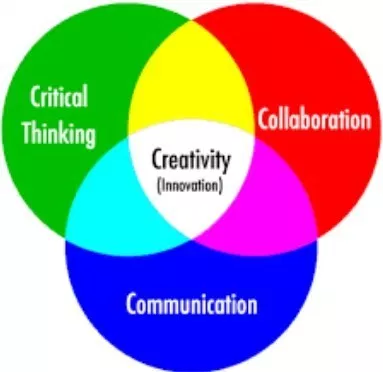
\includegraphics[scale=0.5]{bab1/4C.png}}}
    \caption{\label{fig:1.1}Contoh Gambar}
\end{figure}

\section{Tujuan}


\section{Manfaat}



%%----------------------------------------------------------------------------------------
%%	Bab 2
%%----------------------------------------------------------------------------------------
%\renewcommand{\thetable}{\arabic{chapter}.\arabic{table}}
\renewcommand{\thefigure}{\arabic{chapter}.\arabic{figure}}

\chapter[Gagasan]{\uppercase{Gagasan}}

\setcounter{chapter}{1}
\renewcommand{\thesection}{\norsize\bfseries {\arabic{chapter}.\arabic{section}}}
\titleformat{\section}
{\norsize\bfseries}{\thesection}{1em}{}

\section{Sub Bab 1}

\section{Sub Bab 2}


\section{Sub Bab 3}




%
%%----------------------------------------------------------------------------------------
%%	Bab 3
%%----------------------------------------------------------------------------------------
%\renewcommand{\thetable}{\arabic{chapter}.\arabic{table}}
\renewcommand{\thefigure}{\arabic{chapter}.\arabic{figure}}

\chapter[Simpulan]{\uppercase{Simpulan}}

\setcounter{chapter}{1}
\renewcommand{\thesection}{\norsize\bfseries {\arabic{chapter}.\arabic{section}}}
\titleformat{\section}
{\norsize\bfseries}{\thesection}{1em}{}

\section{Sub Bab 1}

\section{Sub Bab 2}


\section{Sub Bab 3}



%
%
%%----------------------------------------------------------------------------------------
%%	Bab 4
%%----------------------------------------------------------------------------------------
%\input{section/bab4}
%
%
%%----------------------------------------------------------------------------------------
%%	Bab 5
%%----------------------------------------------------------------------------------------
%\input{section/bab5}
%
%
%%----------------------------------------------------------------------------------------
%%	Daftar Pustaka
%%	Jangan mengubah bagian daftar pustaka
%%----------------------------------------------------------------------------------------


\newpage
\setstretch{1.0}  
\setlength{\bibitemsep}{1\baselineskip plus .05\baselineskip minus .05\baselineskip}
\renewcommand{\bibname}{\MakeUppercase{Daftar Pustaka}\\}
\renewcommand*{\bibfont}{\footnotesize}
\xpatchbibmacro{date+extradate}{%
  \printtext[parens]%
}{%
  \setunit{\addperiod\space}%
  \printtext%
}{}{}

\renewcommand{\finalnamedelim}{\addspace\&\space}
\DeclareNameAlias{sortname}{family-given} 
\addcontentsline{toc}{chapter}{\protect\numberline{}{Daftar Pustaka}}
\chapter*{\uppercase{Daftar Pustaka}}
\printbibliography

%----------------------------------------------------------------------------------------
%%	Lampiran
%%----------------------------------------------------------------------------------------
\appendixpage
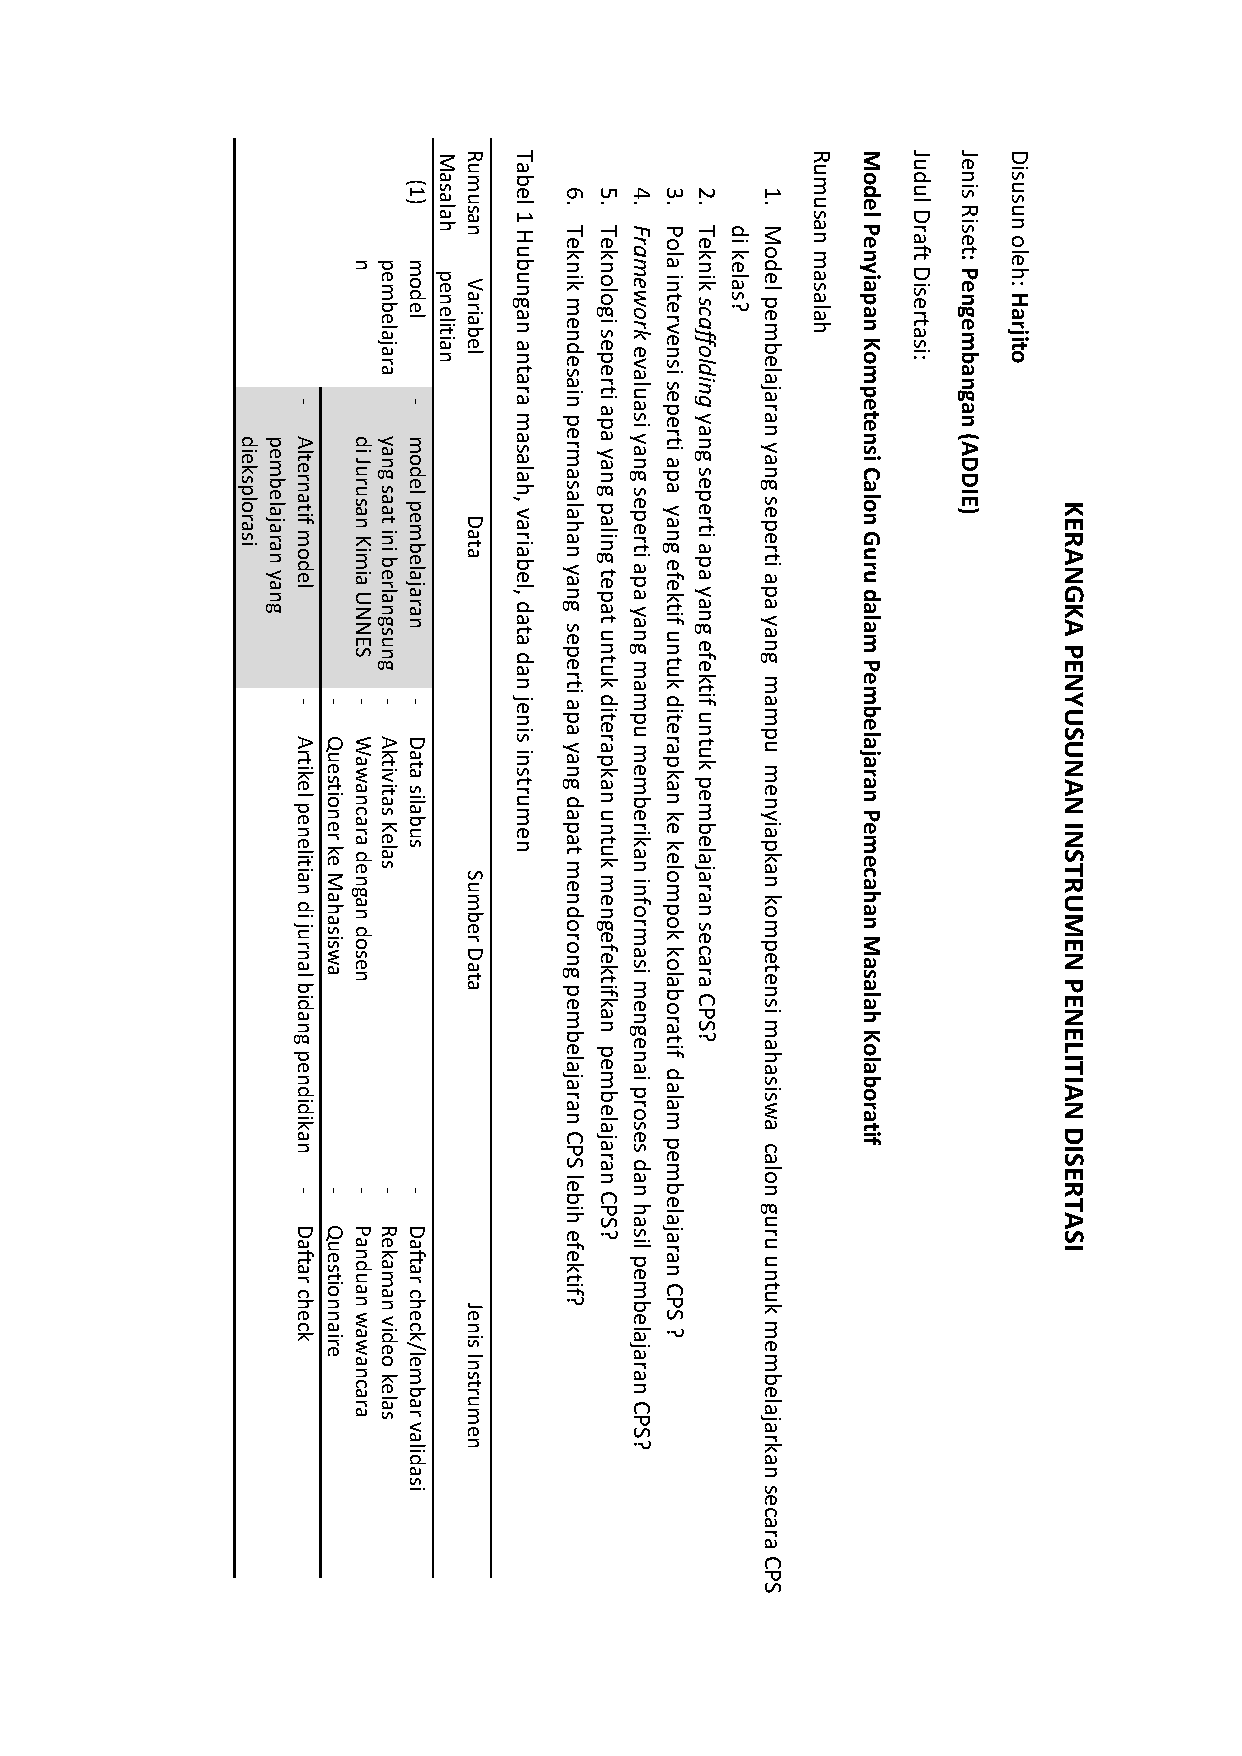
\includepdf[pages=1,scale=0.8,offset=0cm 0cm,pagecommand={
    \begin{flushleft}
        \myappendix{\label{app:1}Data kuesioner}
    \end{flushleft}}]{lampiran/framework-p.pdf}
\includepdf[pages=2-3, scale=0.8, offset=0cm 0cm]{lampiran/framework-p.pdf}    

\end{document}